%-- MOTIVATIONS
\section{Motivations}
\textit{"Why do we choose SSH tunnelling with public keys to implement the security inside the POP-C++ middle-ware ?"}\s

Due to its architecture, a parallel object executed on a node can be contacted on different ports which represent the different protocol implemented for POP-C++. A single node can execute more than one parallel object at the same time. The ports on which the parallel objects will be contacted are not defined before the launching of the application.\s

We needed a security solution that involve the less manipulations on firewalls or existing security installations. The SSH tunnelling provide the SSH security level and need only a single port opened. 


%-- ALTERNATIVES
\pagebreak
\section{Alternatives}
In this chapter, we just summarize some approaches that we have thought about before the implementation. In the future, it could also be implemented inside POP-C++. 

\subsection{TLS(SSL) Combox}
The architecture of POP-C++ let the developer the choice to implement any protocol as a "combox". TLS could be implemented as a combox but there would be a drawback. With TLS, we need to open a lot of ports on firewall and on nodes to let the application execution succeed. In fact, each object running on a node will create its own TLS Server to receive the incoming connections. If we have 20 parallel objects executing on a node, we will need to open 20 ports to let the incoming connections succeed. Due to this, we leave this approach on the side for the moment.

\subsection{SSH with username/password authentication}
A variant of SSH tunnelling using public keys is the username/password authentication. This method could be a little bit less secure because every node executing a parallel object of the application must be initialized with the same username/password pair. On the other side, this method could reduce the traffic generated by the keys exchange. In fact, the interface just need to provide the pair username/password to create the tunnel instead of transfer its key to the node executing the parallel object.


\pagebreak
%-- SSH TUNNELING
\section{SSH Tunnelling}
This chapter aims at introducing the SSH tunnelling and understanding its implication in the POP-C++ middle-ware.

\subsection{What is SSH tunnelling}
The SSH tunnelling allows the creation of a tunnel between a computer running a SSH server and a computer running a SSH client. The tunnel is created between a local destination (address and port) and a remote destination (address and port). All the traffic sent to the local side of the tunnel will be automatically encapsulated into the SSH protocol and sent to the other side of the tunnel. This allows the traffic to pass trough firewalls. In our case, we assume that the port 22 is open on and between computers running POP-C++ in the same GRID infrastructure.

\subsection{Current and desired situation in POP-C++}
In the current version of POP-C++, an interface (the local representative of the parallel object) communicates with the broker (the communication point of the parallel object) through the combox. A combox is an object that implements a specific protocol. When the broker is started, one combox per implemented protocol will be created. Each combox on the broker-side will listen on a different port. The protocol, the address and the port form an access point of the parallel object. This type of connection is illustrated in Figure \ref{fig:std_sec_comm}a.

\begin{figure}[ht]
	\caption{Non-secure and secure connections between the interface and the broker}
  	\centering
	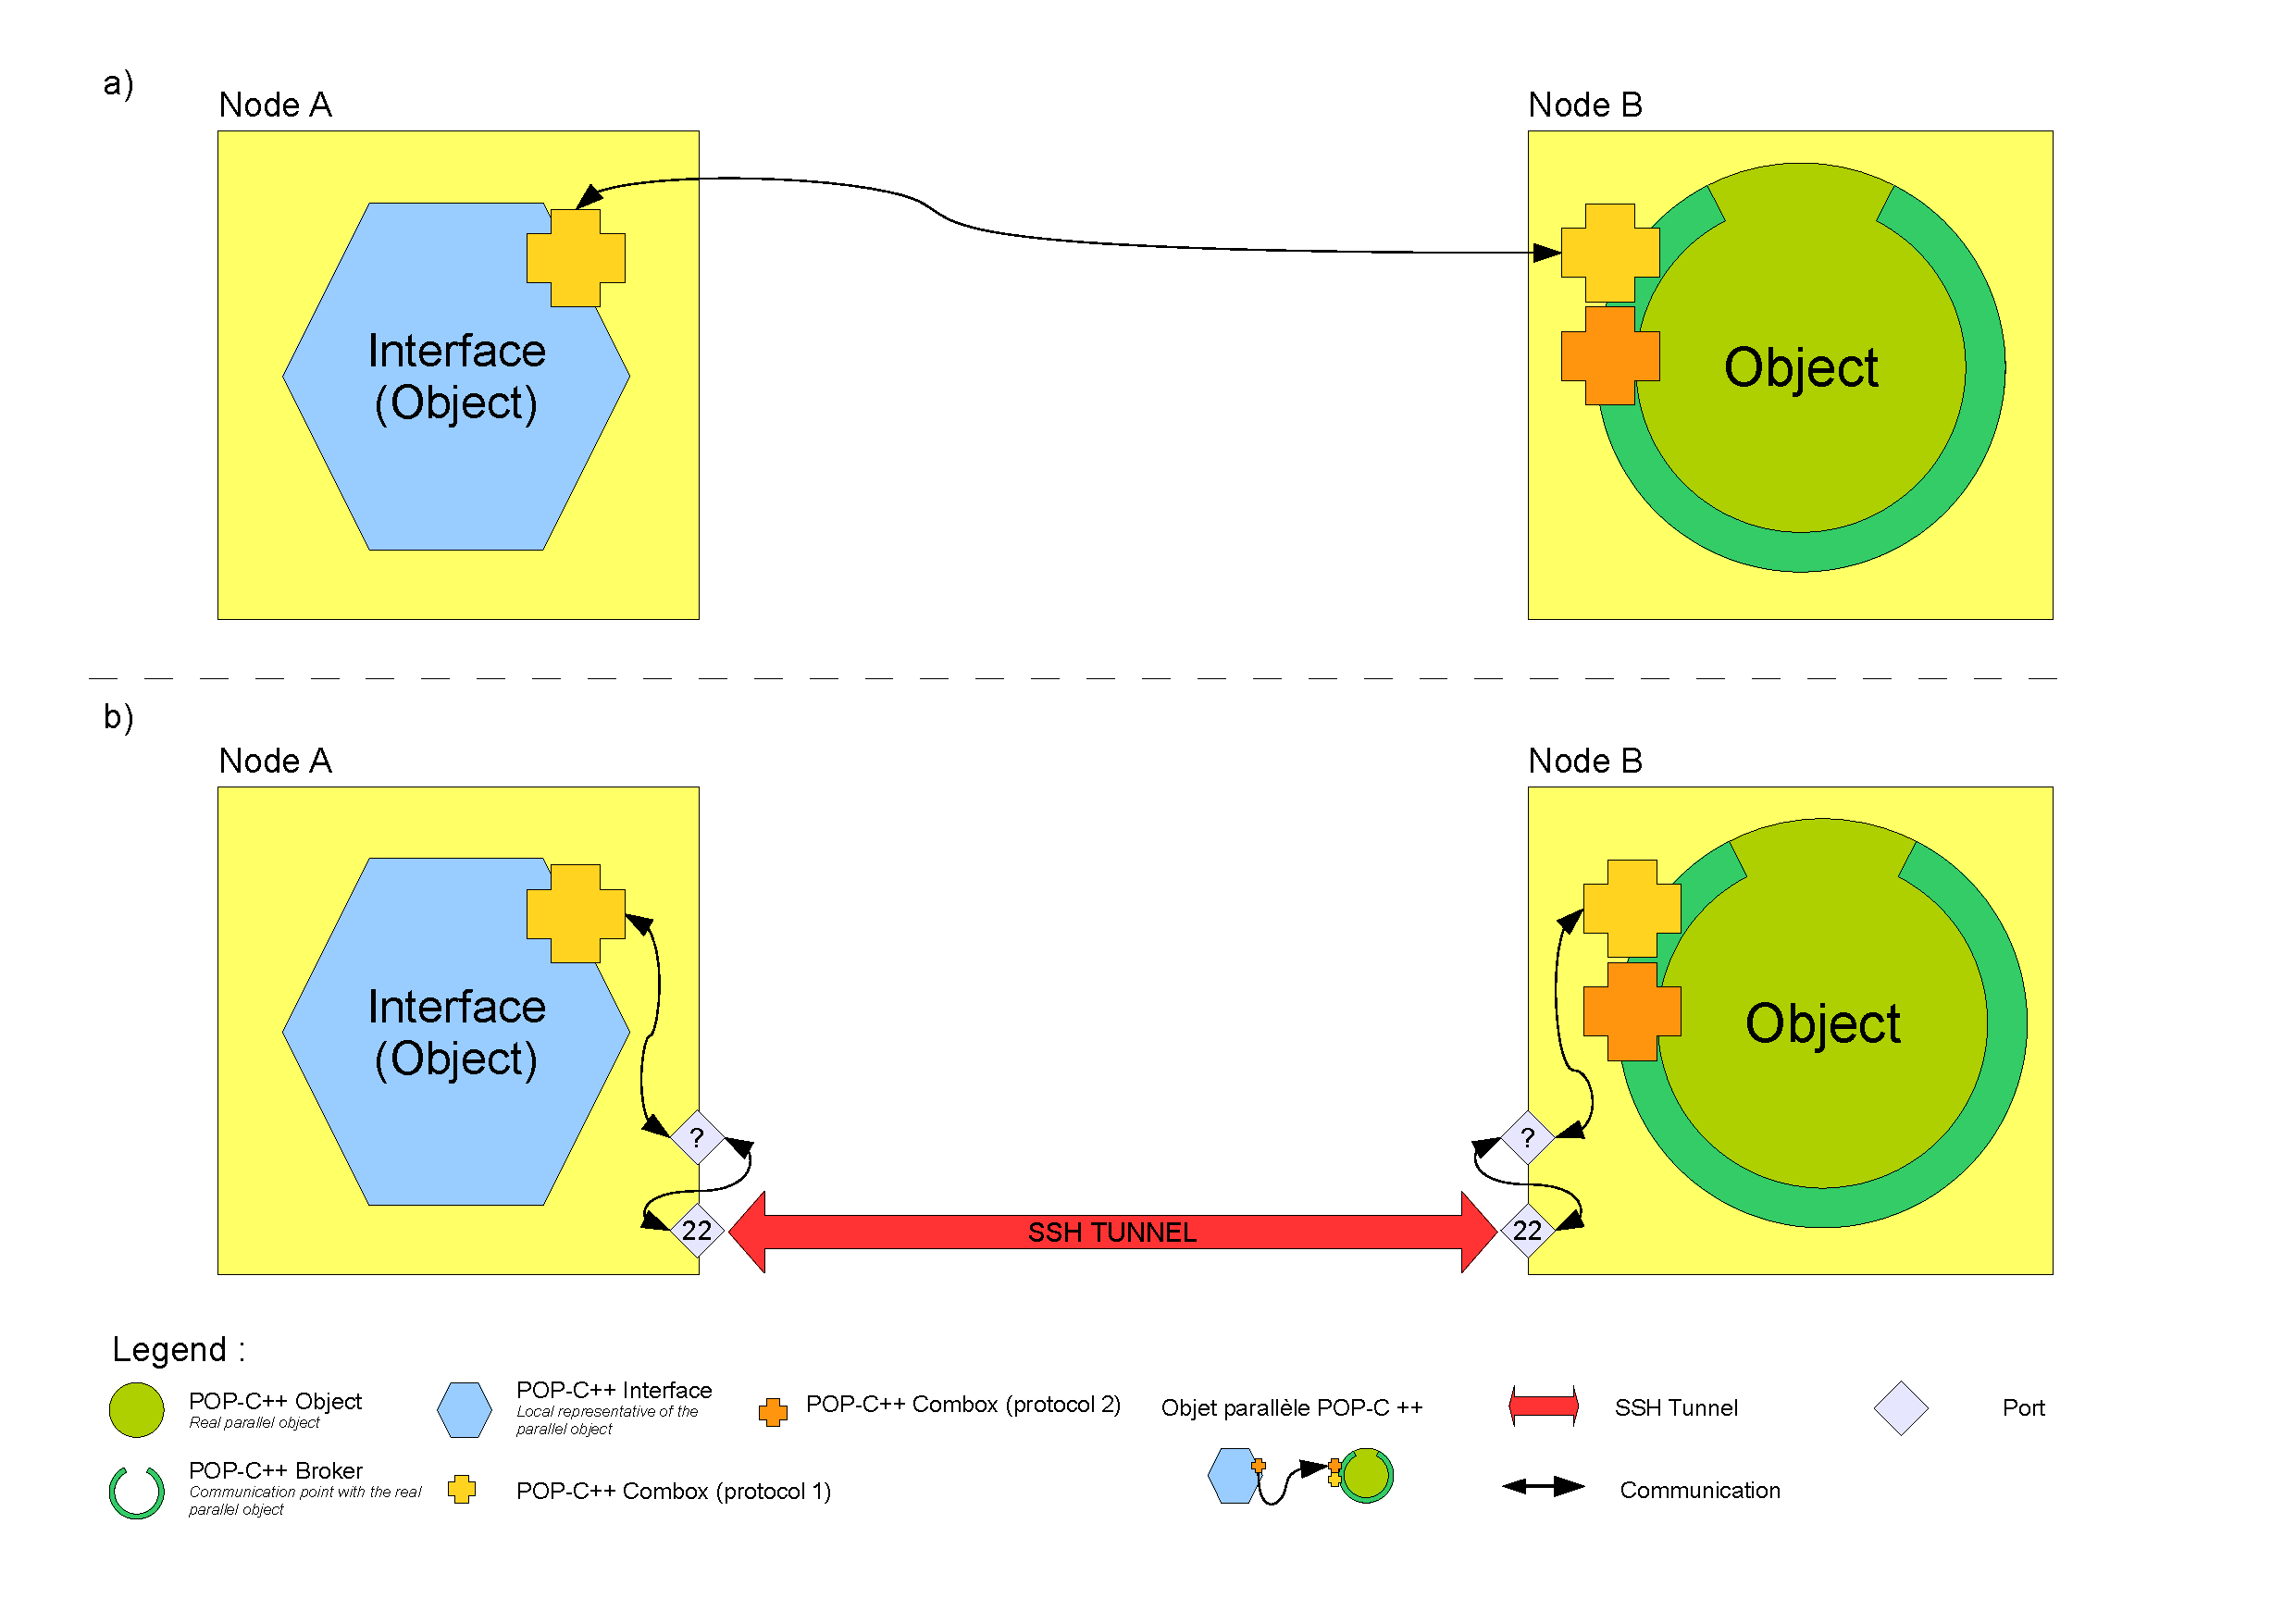
\includegraphics[width=0.9\textwidth]{../std_sec_comm.pdf}
	\label{fig:std_sec_comm}
\end{figure}\vspace{2cm}
\pagebreak

In Figure \ref{fig:std_sec_comm}b, the connection between the interface and the broker is secured by a SSH tunnel. The interface will contact a port on the local machine. This port is redirected through the SSH tunnel to the right remote host address and port.


\subsection{Requirements to use the SSH tunneling}
In order to be able to use the SSH tunneling between an interface and a broker, there are several needs to automatically establish the connection. These needs are listed below : \s
\begin{itemize}
\item The nodes must run a SSH server (e.g. OpenSSH).
\item The port 22 must be opened on the node.
\item If there are any firewalls between nodes, the port 22 must also be opened.
\item The option "StrictHostKeyChecking" must be set to "no". The SSH server will be able to add automatically the new hosts in the file \$HOME/.ssh/known\_hosts.
\item The public key must be exchanged between the two nodes included in a communication.
\end{itemize}\s
The only need that can be done during the installation of POP-C++ is the exchange of the public keys. This exchange process will be explained in Chapter \ref{chap:key_exchange} on page \pageref{chap:key_exchange}.


\subsection{SSH files}
SSH is using public and private keys to authenticate a communication. These keys can be generated with the command \textbf{ssh-keygen}. All the files needed by the SSH process are located in the directory \textbf{\$HOME/.ssh}. This directory contains the following files :  \begin{itemize}
\item \textbf{known\_hosts} : This file stores all the public keys of known nodes.
\item \textbf{id\_rsa} : This file contains the private key. This file must never be exchanged with another node. 
\item \textbf{id\_rsa.pub} : This file contains the public key.
\item \textbf{authorized\_keys} : This file contains the public keys of the nodes that can authenticate automatically to this node.
\end{itemize} 


\subsection{Confidence link in POP-C++}
In order to establish a secure connection between two nodes running POP-C++, they need to have a confidence link between them. This link confirms that one node allows another node to contact him with a secure connection. \\
In our case, the confidence link is established by the exchange of the public SSH keys. Currently, this exchange must be done by hand during the installation of the infrastructure. Only the linked nodes must exchange their key.


